\documentclass[10pt,aspectratio=1609]{beamer}
\usepackage{hyperref}
\usepackage{amsmath}
\usepackage{minted}
\usepackage{venndiagram}
\usepackage{svg}

\usepackage{aneotheme}

\begin{document}
\author{Jérôme Gurhem}
\title{ArmoniK: Simplifying Access to Performance at Scale}
\subtitle{DP2E-AI 2025}
\institute{Aneo}
\date{\today}

\titlepage

\AtBeginSection[]
{
  \frame{\sectionpage}
}

\begin{frame}
  \frametitle{Outline}
  \large
  \tableofcontents
\end{frame}

\newcommand{\vennradius}{2.7cm}
\newcommand{\vennhgap}{2cm}
\newcommand{\vennvgap}{0}
\newcommand{\vennoverlap}{2.1cm}

\begin{section}{Can We Simplify Access to Performance at Scale?}
 \begin{frame}{HPC: At the Cutting Edge of Three Disciplines}
   \begin{center}
     \begin{venndiagram3sets}[labelOnlyA=Software, labelA={}, labelOnlyB=Hardware, labelB={}, labelOnlyC={Scientific Problem to Solve}, labelC={}, labelABC={HPC}, showframe=false, radius=\vennradius, hgap=\vennhgap, vgap=\vennvgap, overlap=\vennoverlap]
       \fillACapBCapC
     \end{venndiagram3sets}
   \end{center}
 \end{frame}

 \begin{frame}
   \frametitle{The Decline of the Scientific Polymath}

   \begin{itemize}
     \item \textbf{17th–18th centuries:} Scientists like Newton and Leibniz contributed across disciplines — science was relatively unified.
     \item \textbf{19th century:} Rapid growth of disciplines (e.g., chemistry, biology, physics); first signs of specialization.
     \item \textbf{20th century:} Explosion of subfields and technical complexity; solo mastery becomes impossible.
     \item \textbf{Today:} Even within a single field (e.g., AI, genetics), experts specialize narrowly — cross-field comprehension is rare.
   \end{itemize}

   \begin{block}{Result}
     \begin{itemize}
       \item No one scientist can read or understand all scientific publications.
       \item Applicable to HPC : It is increasingly difficult to master all its fields.
     \end{itemize}
   \end{block}
 \end{frame}

 \begin{frame}{Building Interfaces Between Disciplines}
   \begin{center}
     \begin{venndiagram3sets}[labelOnlyA=Software, labelA={}, labelOnlyB=Hardware, labelB={}, labelOnlyC={Scientific Problem to Solve}, labelC={}, labelABC={HPC}, labelOnlyAB={Compilers}, labelOnlyBC=\parbox{2cm}{ASIC, FPGA, Tensor Cores}, labelOnlyAC={Libraries}, showframe=false, radius=\vennradius, hgap=\vennhgap, vgap=\vennvgap, overlap=\vennoverlap]
       \fillACapBCapC
     \end{venndiagram3sets}
   \end{center}
 \end{frame}

 \begin{frame}{Current Interfaces}
   \begin{itemize}
     \item \textbf{Hardware/Software}
           \begin{itemize}
             \item \textbf{Programming Languages:} C, C++, Python, Fortran, etc.
             \item \textbf{Compilers:} GCC, Intel, LLVM, etc.
           \end{itemize}
     \item \textbf{Software/Scientific Problem}
           \begin{itemize}
             \item \textbf{Libraries:} BLAS, LAPACK, FFTW, TensorFlow, PyTorch, etc.
             \item \textbf{Frameworks:} MPI, OpenMP, CUDA, OpenCL, Kokkos, etc.
           \end{itemize}
     \item \textbf{Hardware/Scientific Problem}
           \begin{itemize}
             \item \textbf{AI:} AWS Inferentia, Google TPU, Nvidia Tensor Cores, etc.
             \item \textbf{Dedicated Accelerators:} FPGAs, ASICs, etc.
           \end{itemize}
   \end{itemize}
   \pause
   \begin{alertblock}{Are they good enough?}
     \begin{itemize}
       \item Yes ! For the trade-off they were designed for.
       \item Still, they need deep expertise to be used effectively.
     \end{itemize}
   \end{alertblock}
 \end{frame}

 \begin{frame}{Why Look Beyond Current Interfaces?}
   \begin{itemize}
     \item Complexity of heterogeneous systems is growing rapidly.
     \item Experts are required to bridge hardware/software/application gaps.
     \item Scientific applications need:
           \begin{itemize}
             \item Scalability without re-architecting code.
             \item Transparent access to diverse computing resources.
             \item Efficient resource utilization and orchestration.
           \end{itemize}
     \item Current solutions lack:
           \begin{itemize}
             \item Flexibility across architectures.
             \item Seamless integration and automation.
             \item User-friendly interfaces for scientists and engineers.
           \end{itemize}
   \end{itemize}
   \pause
   \begin{block}{The Question}
     Can we simplify access to performance at scale?
   \end{block}
 \end{frame}
\end{section}

\begin{section}{ArmoniK: A User-Friendly Trade-Off}
 \begin{frame}
   \frametitle{ArmoniK's Goals}
   \begin{itemize}
     \item Simplify the development of distributed applications
     \item Provide a user-friendly interface for scientists and engineers
     \item Adress the challenges of HPC without requiring deep expertise in parallel programming
     \item Getting reasonable performances
   \end{itemize}
 \end{frame}

 \begin{frame}
   \frametitle{ArmoniK: a Hybrid Framework}
   \includegraphics[width=\textwidth]{armonik_framework.pdf}
   \begin{itemize}
     \item Computational kernels: User computations
     \item Data management: Reads, Writes, Communications between processes
     \item Advanced features: Overlapping, load balancing
     \item Jobs management: Job queues, resource allocation, job lifecycle
     \item Jobs / Resources mapping: Determine job execution on which machines
     \item Resources management: Machine pool update, node addition or removal
   \end{itemize}
 \end{frame}

 \begin{frame}
   \frametitle{Task-based Programming in ArmoniK}
   \begin{block}{Definition}
     Paradigm focusing on the decomposition of complex operations into smaller tasks
   \end{block}
   \begin{itemize}
     \item Expression of complex data-driven dependencies
     \item ArmoniK's \textbf{distributed scheduler} responsible for:
           \begin{itemize}
             \item Task distribution and load balancing
             \item Dependency resolution
             \item Tasks execution
             \item Data management (overlapping, prefetching, and checkpointing)
           \end{itemize}
   \end{itemize}
   \vskip1ex
   \footnotesize
   \inputminted[frame=single]{python}{task-based-programming.py}
 \end{frame}

 \begin{frame}
   \frametitle{ArmoniK Programming Model}
   \begin{columns}[T]
     \begin{column}{0.5\textwidth}
       \begin{itemize}
         \item \textbf{Task Graph}: Bipartite DAG whose node sets are tasks and data
         \item \textbf{Task node}: Single-node computation (possibly multi-threaded) taking one or several data inputs and outputting one or several data
         \item \textbf{Data node}: Immutable piece of data depending on only one task at most
         \item \textbf{Dependencies}: Dependencies between tasks are expressed as data dependencies
         \item \textbf{Dynamic}: The graph may not be entirely known in advance (tasks can append tasks and replace edges with subgraphs)
       \end{itemize}
     \end{column}
     \begin{column}{0.5\textwidth}
       \centering
       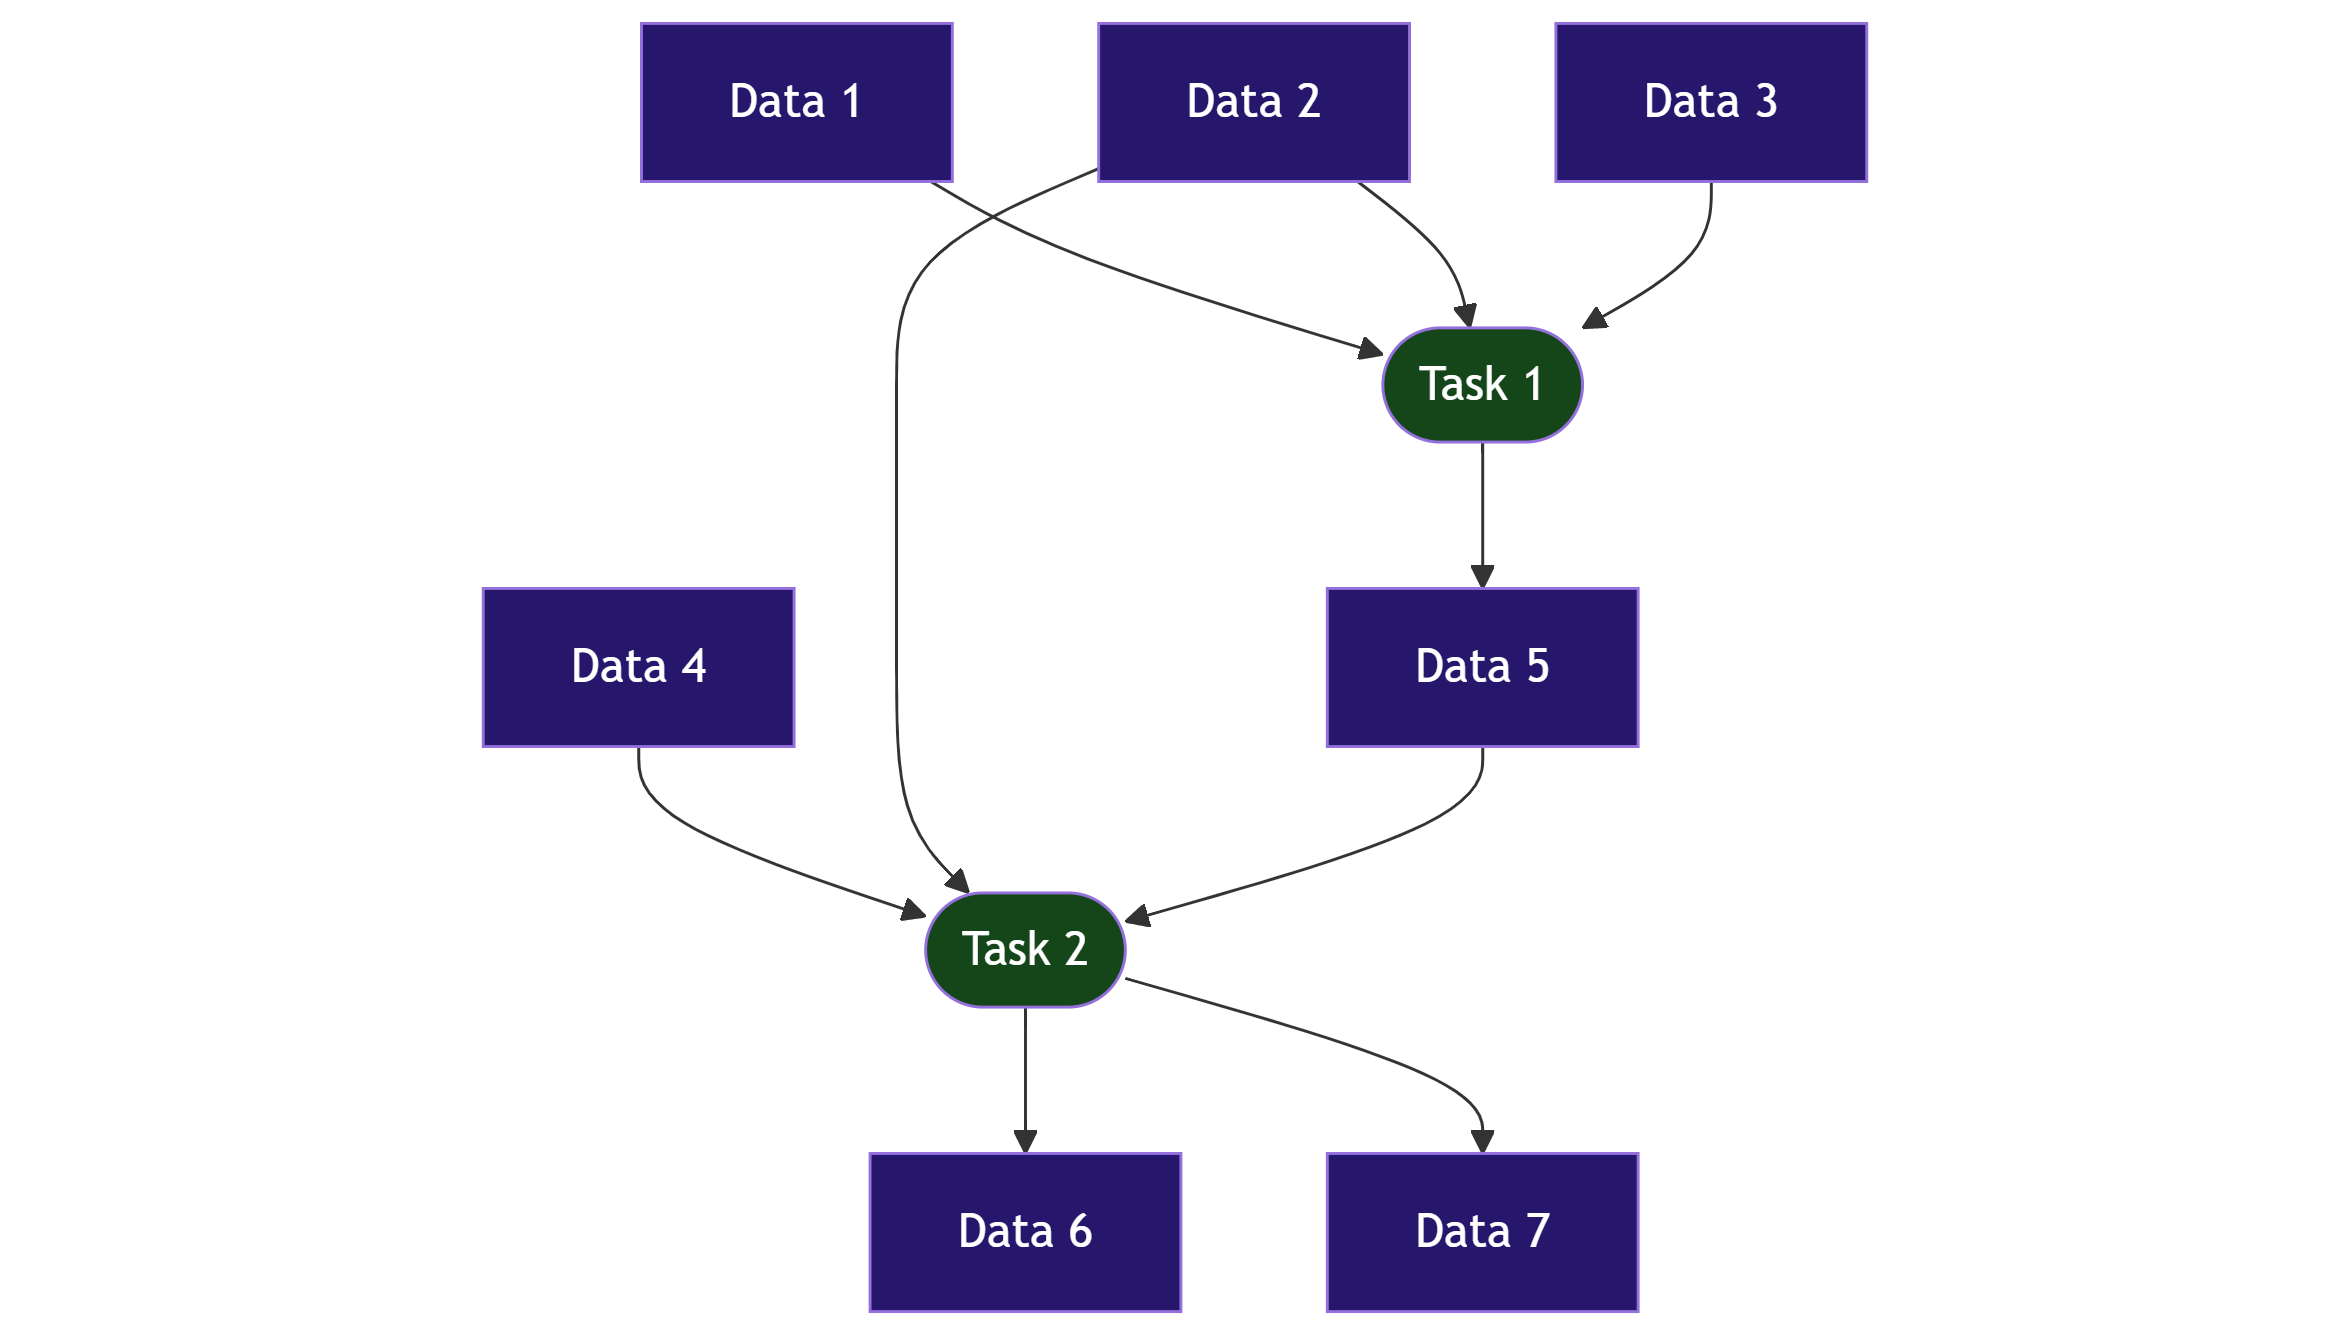
\includegraphics[width=0.95\textwidth]{mermaid-task-graph.png}
     \end{column}
   \end{columns}
 \end{frame}

 \begin{frame}
   \frametitle{Dynamic Graph}
   \begin{block}{Definition}
     Dependency graph is not fully known when scheduling starts.
   \end{block}
   \begin{itemize}
     \item Task dependencies not known before submission
     \item Submissions can happen anytime
     \item Tasks can submit new tasks
     \item Tasks can delegate the production of their output to their new tasks
   \end{itemize}
   \footnotesize
   \inputminted[frame=single]{python}{subtasking.py}
 \end{frame}

 \begin{frame}
   \frametitle{Dynamic Graph Example}
   \begin{figure}
     \includesvg[width=0.8\textwidth]{subtasking.svg}
   \end{figure}
 \end{frame}

 \begin{frame}
   \frametitle{Computations/Comm Overlapping}
   \begin{block}{Data Management}
     Responsibility for data allocation, transfer, and storage between computational operations
   \end{block}
   \begin{itemize}
     \item ArmoniK is responsible for tasks input and output data management
     \item Allows for automatic communication + scheduling/task execution overlapping
     \item Automatic Uncoordinated Checkpointing
   \end{itemize}
   \begin{figure}
     \includegraphics[width=0.8\textwidth, trim={0 7cm 0 0}, clip]{pipelining AK 2.pdf}
   \end{figure}
 \end{frame}

 \begin{frame}
   \frametitle{ArmoniK Built-in Features}
   \begin{itemize}
     \item \textbf{Open Source}: \url{https://github.com/aneoconsulting/ArmoniK}
     \item \textbf{Observability}: Extensive GUIs, CLIs, monitoring APIs, metrics, logs, and traces
     \item \textbf{Portability}: Effort to transfer an application from one environment to another
           \begin{itemize}
             \item Officially supported languages: C\#, C++, Python, Rust, Java, and JavaScript
             \item Tasks on different architectures (x86, ARM, GPU, Linux, Windows), applications, environments
           \end{itemize}
     \item \textbf{Malleability}: Dynamic reconfiguration of the number of allocated resources during execution without interruption
     \item \textbf{Resource Sharing}: Share resources between applications to maximize resource utilization
     \item \textbf{Modularity}: Modules can be swapped without modifying ArmoniK's code to suit user needs and constraints
     \item \textbf{Production Ready}: Designed to be used in production environments, with a focus on stability, security, scalability, and maintainability
           \begin{itemize}
             \item Used by our clients in their critical systems
             \item Drives our needs for validation and guarantees, monitoring, stability
           \end{itemize}
   \end{itemize}
 \end{frame}

 \begin{frame}
   \frametitle{Fault Tolerance}
   \begin{itemize}
     \item Works without interruption even when one or more nodes fail
     \item Allow support for preemptible computing resources
     \item Automatic and efficient task retry on failure
     \item Each curve represents a percentage of preempted instances
   \end{itemize}
   \begin{center}
     \vspace{0.2ex}
     \includesvg[width=0.75\textwidth]{bench_preemption.svg}
   \end{center}
 \end{frame}

 \begin{frame}
   \frametitle{Throughput Scalability}
   \begin{itemize}
     \item Indep : independent tasks workload
     \item Graph : nested fork-join workload
     \item 1-second long tasks
     \item Empty input/output data
   \end{itemize}
   \begin{center}
     \includesvg[width=0.8\textwidth]{bench_scalability.svg}
   \end{center}
 \end{frame}

 \begin{frame}
   \frametitle{Low Round-trip Latency}
   \begin{itemize}
     \item Cumulative distribution functions (CDFs) of round-trip latency
     \item Batched submissions of 1, 10, and 100 independent zero-work tasks
   \end{itemize}
   \begin{center}
     \includesvg[width=0.8\textwidth]{bench_roundtrip_latency.svg}
   \end{center}
 \end{frame}

\end{section}

\begin{section}{Towards AI with ArmoniK and JAX}
 \begin{frame}
   \frametitle{JAX: A Modern Tool for Scientific Computing and AI}
   \textbf{JAX} is a Python library that enables high-performance scientific computing by combining:
   \begin{itemize}
     \item \textbf{NumPy-Compatible API} for familiar, concise numerical code
     \item \textbf{Automatic differentiation} for optimization and ML
     \item \textbf{Just-In-Time (JIT) compilation} for accelerating performance
     \item \textbf{Seamless CPU, GPU, and TPU execution}
     \item \textbf{Composable Transformations} Combine transformations easily: e.g., \texttt{jit(grad(f))}, \texttt{vmap(grad(f))}.
   \end{itemize}
 \end{frame}

 \begin{frame}
   \frametitle{XLA: The Compiler Behind the Speed}
   \begin{itemize}
     \item \textbf{XLA (Accelerated Linear Algebra)} is a domain-specific compiler developed by Google.
     \item It transforms JAX Python functions into highly optimized machine code.
     \item Performs \textbf{operation fusion, memory planning, and hardware-specific optimizations}.
     \item Enables JAX to deliver \textbf{hardware-level performance} from high-level Python code.
     \item Produces efficient code for CPUs, GPUs, and TPUs.
   \end{itemize}
 \end{frame}

 \begin{frame}
   \frametitle{Impact for Scientists and Engineers}
   \begin{itemize}
     \item Write portable, optimized code without low-level programming
     \item Accelerate AI models, PDE solvers, and simulation kernels
     \item Integrate HPC workflows with modern ML toolchains
     \item Reduces boilerplate in high-performance computing
     \item Enables reproducible, portable, and efficient scientific models
   \end{itemize}
 \end{frame}

 \begin{frame}
   \frametitle{ArmoniK + JAX: A Powerful Combination}
   \begin{itemize}
     \item \textbf{ArmoniK} provides a distributed task scheduler and data management layer.
     \item \textbf{JAX} offers high-performance numerical computing capabilities.
     \item Together, they enable:
           \begin{itemize}
             \item Scalable, fault-tolerant AI and scientific computing
             \item Automatic data management and task scheduling
             \item Efficient execution on heterogeneous hardware
           \end{itemize}
     \item Ideal for large-scale AI training, scientific simulations, and data analysis.
     \item Supports dynamic task graphs and overlapping computations.
     \item Provides a user-friendly interface for scientists and engineers.
   \end{itemize}
 \end{frame}

 \begin{frame}
   \frametitle{What It Looks Like}
   \begin{itemize}
     \item Ideal for large-scale AI training, scientific simulations, and data analysis.
           \inputminted[breaklines,frame=single,fontsize=\small]{python}{cholesky_simple.py}
     \item Use GPUs instead of CPUs, just swap dependencies and partition.
           \inputminted[breaklines,frame=single,fontsize=\small]{python}{cholesky_simple_gpu.py}
           %  \item Also works for TPUs.
           %  \item The JAX Neuron library allows to use AWS Trainium and Inferencia chips.
   \end{itemize}
 \end{frame}
\end{section}

\begin{section}{The Right Tool for the Right Job}
 \begin{frame}
   \frametitle{The Right Tool for the Right Job}
   \begin{itemize}
     \item No single scientist can master all fields in HPC.
     \item Interfaces between disciplines are crucial.
     \item And the trade-off between performance and usability is essential.
     \item However, the current trade-off is speed-oriented, requiring deep expertise.
     \item ArmoniK aims to shift this trade-off towards usability while maintaining reasonable performance.
     \item It allows scientists to focus on their research without needing deep expertise in parallel programming.
     \item ArmoniK is not a replacement for existing HPC tools but a complementary framework that simplifies the development of distributed applications.
     \item We are looking for more use cases: \url{https://github.com/aneoconsulting/ArmoniK}
   \end{itemize}
 \end{frame}

 \begin{frame}
   \frametitle{Questions and Discussions}
   \begin{itemize}
     \item What missing interoperability layers (software, standard, or abstraction) would most accelerate convergence between traditional HPC linear algebra workflows and today's extreme-scale AI workloads?
           \begin{itemize}
             \item There are tentatives between hardware and software (Kokkos, JAX, etc.), but what about applications that does not fit in these frameworks?
             \item In companies, we see that over time, organizational interfaces tends to match the interfaces in the IT systems.
             \item We still have a lot of work to build scientific and technology interfaces that allows users to cooperate without a deep expertise in all HPC/AI-related fields.
           \end{itemize}
     \item Looking ahead to 2030, do you expect the principal bottleneck for extreme-scale AI to be data, algorithms, resilience or energy, and how does that prediction shape your research priorities today?
           \begin{itemize}
             \item \textbf{Energy}: It will probably be an issue in Europe, probably less true elsewhere.
             \item It will be a trade-off between the three others.
           \end{itemize}
     \item Given the different developments in architecture processors for AI and “computational science”, do you think we'll see a convergence or divergence of roadmaps?
           \begin{itemize}
             \item HPC will use whatever will be available on the market, as in the last 30 years.
           \end{itemize}
   \end{itemize}
 \end{frame}

 \begin{frame}
   \frametitle{Thank you for your attention!}
   Do you have any questions?
 \end{frame}
\end{section}

\end{document}